\ccParDims

\ccUserChapter{2D Boolean Operations on Nef Polygons Embedded on the Sphere  \label{chapterNef_S2}}

\ccChapterRelease{\Nef_polyhedron_S2Rev. \ \Nef_polyhedron_S2Date}
\ccChapterAuthor{Peter Hachenberger \and Lutz Kettner}



\begin{ccPkgDescription}{3D Convex Hulls\label{Pkg:ConvexHull3}}
\ccPkgHowToCiteCgal{cgal:hs-ch3-07}
\ccPkgSummary{This package provides functions 
for computing convex hulls in three dimensions as well as functions
for checking if sets of points are strongly convex are not. One can
compute the convex hull of a set of points in three dimensions in one
of three ways: using a static algorithm, using an incremental
construction algorithm, or using a triangulation to get a fully
dynamic computation.}

\ccPkgDependsOn{All algorithms produce as output a \ccRef[3D Polyhedron]{Pkg:Polyhedron}. 
                The dynamic algorithms depend on \ccRef[3D Triangulations]{Pkg:Triangulation3}}
\ccPkgIntroducedInCGAL{1.1}
\ccPkgLicense{\ccLicenseQPL}
\ccPkgIllustration{Convex_hull_3/bunny.png}{Convex_hull_3/bunny.png}
\end{ccPkgDescription}


\minitoc

% +========================================================================+
\section{Introduction}
% +========================================================================+

Nef polyhedra are defined as a subset of the d-dimensional space obtained by
a finite number of set complement and set intersection operations on
halfspaces. 

Due to the fact that all other binary set operations like union,
difference and symmetric difference can be reduced to intersection and
complement calculations, Nef polyhedra are also closed under those
operations. Also, Nef polyhedra are closed under topological unary 
set operations. Given a Nef polyhedron one can determine its interior, its
boundary, and its closure.

\begin{figure}[htbp]
\begin{ccTexOnly}
\begin{center}
\scalebox{0.5}{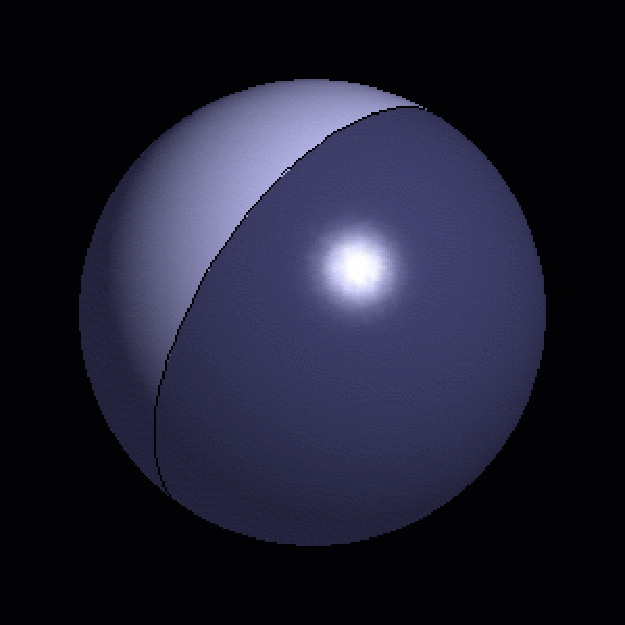
\includegraphics{Nef_S2/fig/halfspace}}
\hspace{1cm}
\scalebox{0.5}{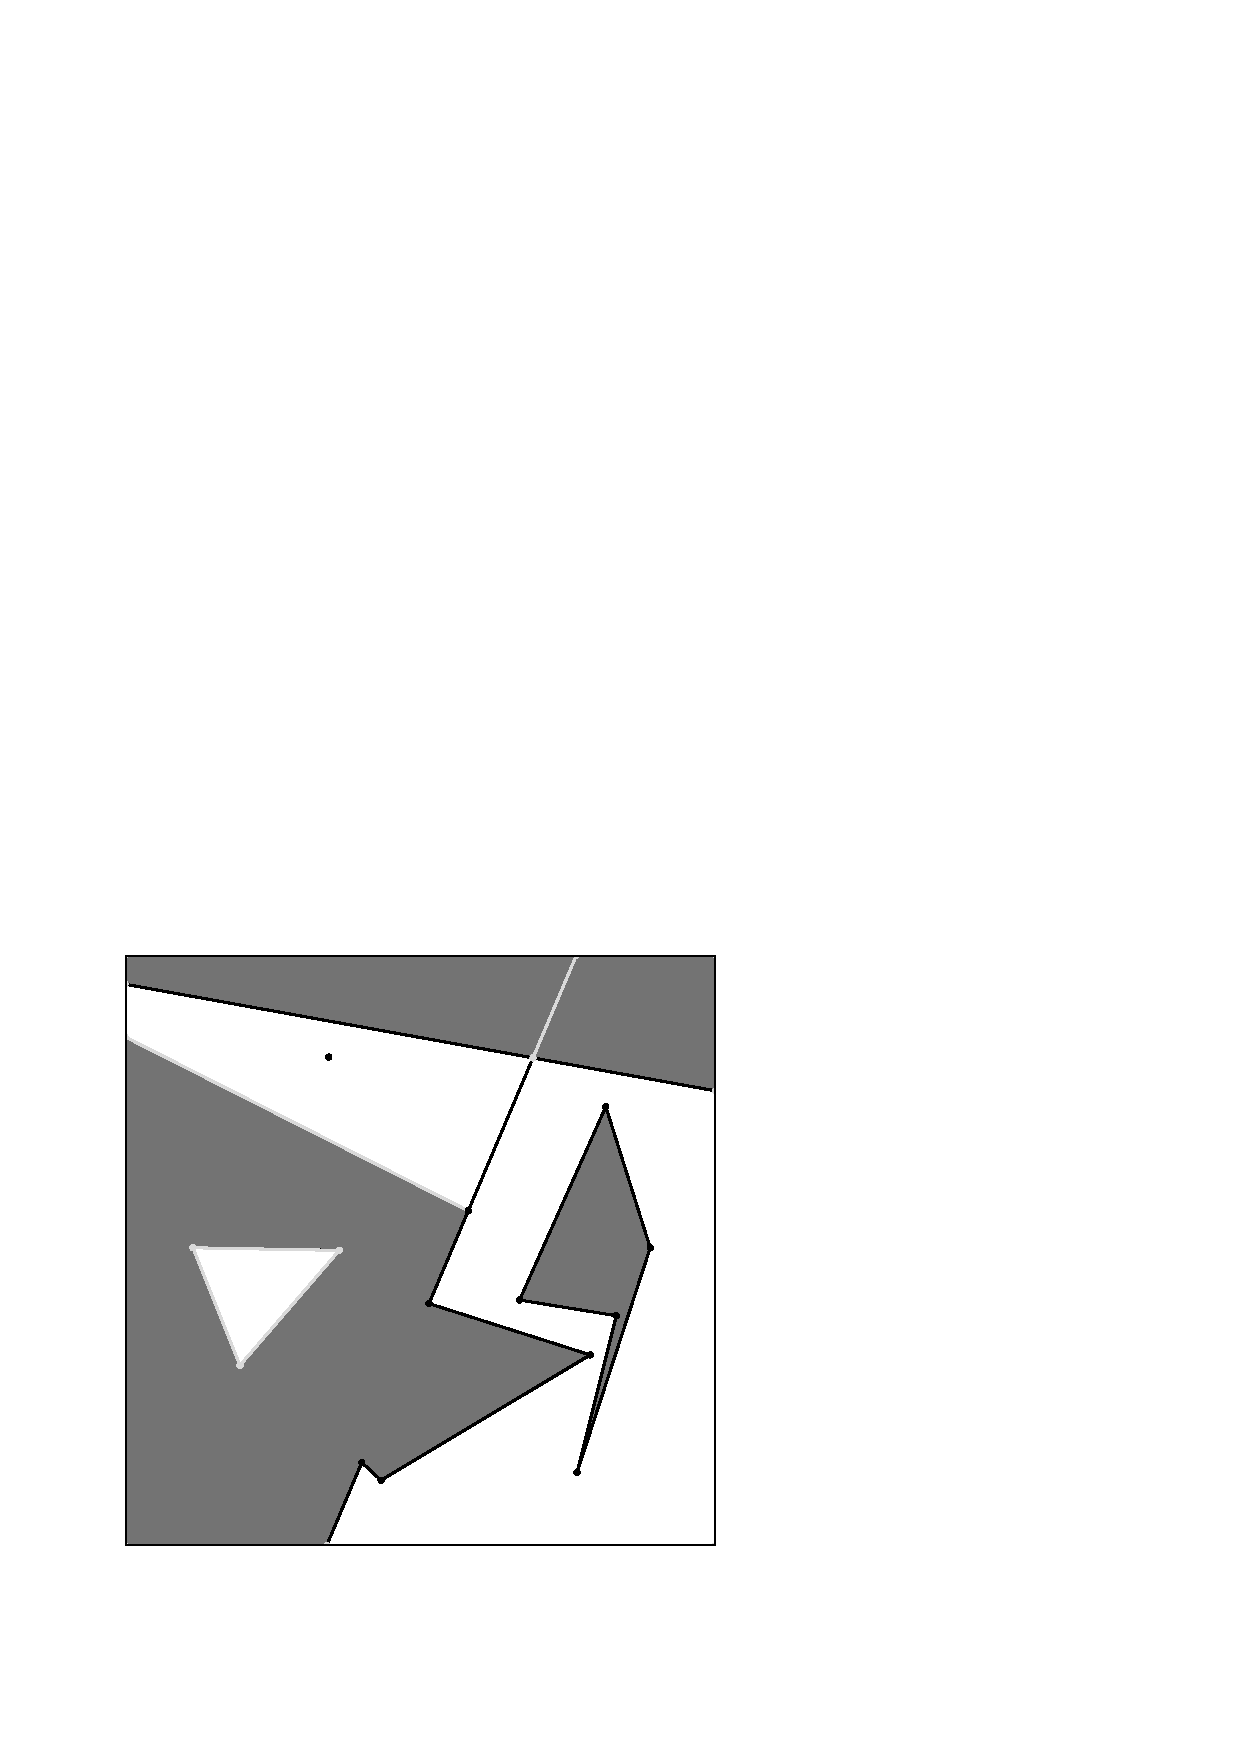
\includegraphics{Nef_S2/fig/complex}}
\end{center}
\end{ccTexOnly}
\caption{Two spherical Nef polyhedra. A closed halfspace on the left 
  and a complex polyhedron on the right. The different colors indicate
  selected and unselected regions, lines and points.}\label{nefsexamples}
\begin{ccHtmlOnly}
<CENTER>
<IMG BORDER=0 SRC="fig/halfspace.gif" ALIGN=middle
ALT="a halfplane">
<IMG BORDER=0 SRC="fig/complex.gif" ALIGN=middle
ALT="a complex polyhedron">
</CENTER>
\end{ccHtmlOnly}
\end{figure}      

Additionally, a d-dimensional Nef polyhedron has the property, that its boundary
is a (d-1)-dimensional Nef polyhedron. This property can be used as a way to
represent 3-dimensional Nef polyhedra by means of planar Nef polyhedra.
This is done by intersecting the neighborhood of a vertex in a 3D Nef polyhedron
with an $\epsilon$-sphere. The result is a planar Nef polyhedron embedded
on the sphere.

The intersection of a halfspace going through the center of the $\epsilon$-sphere,
with the $\epsilon$-sphere, results in a halfsphere which is bounded by
a great circle. A binary operation of two halfspheres cuts the great circles
into great arcs.

\begin{ccTexOnly}
    \vspace{-7mm}
    \begin{center}
      \parbox{0.4\textwidth}{%
          \includegraphics[width=0.4\textwidth]{Nef_S2/fig/shalfloopB}%
      }
    \end{center}
    \vspace{-5mm}
\end{ccTexOnly}

\begin{ccHtmlOnly}
    <CENTER>
    <A HREF="./fig/shalfloopB.gif">
        <img src="./fig/shalfloopB.gif" alt="SHalfloop Diagram"></A><P>
    </CENTER>
\end{ccHtmlOnly}

The incidence structure of planar Nef polyhedra can be reused. The items
are denoted as $svertex$, $shalfedge$ and $sface$, analogous 
to their counterparts in \ccc{Nef_polyhedron_S2}. Additionally, there is the
\emph{shalfloop} reprsenting the great circles. The incidences are 
illustrated in the figure above.

\section{Restricted Spherical Geometry}

We introduce geometric objects that are part of the spherical surface
$S_2$ and operations on them. We define types \ccc{Sphere_point},
\ccc{Sphere_circle}, \ccc{Sphere_segment}, and \ccc{Sphere_direction}.
\ccc{Sphere_point}s are points on $S_2$, \ccc{Sphere_circle}s are
oriented great circles of $S_2$, \ccc{Sphere_segment}s are oriented
parts of \ccc{Sphere_circles} bounded by a pair of
\ccc{Sphere_point}s, and \ccc{Sphere_direction}s are directions that
are part of great circles. (a direction is usually defined to be a
vector without length, that floats around in its underlying space and
can be used to specify a movement at any point of the underlying
space; in our case we use directions only at points that are part of
the great circle that underlies also the direction.)

Note that we have to consider special geometric properties of the
objects. For example two points that are part of a great circle define
two \ccc{Sphere_segment}s, and two arbitrary \ccc{Sphere_segment}s can
intersect in two points.

If we restrict our geometric objects to a so-called perfect hemisphere
of $S_2$\footnote{A perfect hemisphere of $S_2$ is an open half-sphere
  plus an open half-circle in the boundary of the open half-sphere
  plus one endpoint of the half-circle.} then the restricted objects
behave like in classical geometry, e.g., two points define exactly one
segment, two segments intersect in at most one interior point
(non-degenerately), or three non-cocircular sphere points can be
qualified as being positively or negatively oriented.

% +========================================================================+
\section{Example Programs}
% +========================================================================+
\label{sectionNef_S2Examples}

% +------------------------------------------------------------------------+
\subsection{First Example}

In this first example \ccc{Nef_polyhedron_S2} is parametrized with a CGAL
Kernel as traits class. The types comprising the spherical geometry can be
retrieved from the type \ccc{Nef_polyhedron_S2<Traits>} as is done in the example 
with the type
\ccc{Sphere_circle}. Then three Nef polyhedra are created: $N1$ is a halfsphere
including the boundary, $N2$ is another halfsphere without the boundary, and 
$N3$ is the intersection of $N1$ and $N2$. 

\ccIncludeExampleCode{Nef_S2/simple.cpp}

% +------------------------------------------------------------------------+
\subsection{Construction and Combinations}

Th example shows the different types of constructors: $N1$ is the complete
sphere, $N2$ is a halfsphere which includes the boundary, $N3$ is created
with the copy constructor, $N4$ is created as an arrangement of a set
of \ccc{Sphere_segments}, and $N5$ is created as the empty set.

The example also shows the use of unary set operations, binary operations, 
and binary predicates: $N3$ is defined as the complement of $N2$, $N1$ is
compared with the union of $N2$ and $N3$, $N5$ is united with $N2$ and then
intersected with $N4$. At last, it is tested if $N5$ is a subset of $N2$ and
if $N5$ is not equal to $N4$. 

\ccIncludeExampleCode{Nef_S2/nef_s2_construction.cpp}

% +------------------------------------------------------------------------+
\subsection{Exploration}

By recursively composing binary and unary operations one can end with
a very complex rectilinear structure. \ccc{Nef_polyhedron_S2} allows 
read-only exploration of the structure.

In the following example, a random \ccc{Nef_polyhedron_S2 S} created from
\ccc{n} halfspheres is explored. Each sface is composed of one outer 
sface cycles and an arbitrary number of inner sfaces cycles. The outer cycle
is either an shalfloop or a cycle of shalfedges. An inner cycles additionally
can be an isolated vertex. The example shows how to get the entry item \ccc{it}
to all sface cycles of an sface \ccc{sf} and how to find out what type of item
it is. 

The macro \ccc{CGAL_forall_sface_cycles_of} is equivalent to a for-loop
on the range \ccc{[sf->sface_cycles_begin(), sf->sface_cycles_end())}. An 
\ccc{SFace_cycle_const_iterator} either represents a \ccc{SVertex_const_handle},
a \ccc{SHalfede_const_handle} or a \ccc{SHalfloop_const_handle}. In order
to find out which handle type is represented, the functions
\ccc{is_svertex()}, \ccc{is_shafledge()} and \ccc{is_shalfloop()} are provided.
Afterwards the iterator can be casted to the proper handle type.

\ccIncludeExampleCode{Nef_S2/nef_s2_exploration.cpp}

% +------------------------------------------------------------------------+
\subsection{Point Location}

Using the \ccc{locate} function, it is possible to retrive an item at a
certain location on the sphere. In the following example, the item at 
location \ccc{Sphere_point(1,0,0)} in a random \ccc{Nef_polyhedron_S2} is 
retrieved. \ccc{locate} returns an instance of type \ccc{Object_handle}, which
is a container for any handle type. Here, it  either a 
\ccc{SVertex_const_handle}, a \ccc{SHalfedge_const_handle}, 
a \ccc{SHafloop_const_handle} or a \ccc{SFace_const_handle}. The function 
\ccc{CGAL::assign} performs the cast operation and returns a boolean which
indicates whether the cast was successful or not.

\ccIncludeExampleCode{Nef_S2/nef_s2_point_location.cpp}


% +------------------------------------------------------------------------+
\subsection{Visualization}


\ccc{Nef_polyhedron_S2} provides an interface for OpenGL visualization via a
Qt widget. The usage is shown in the following example:

\ccIncludeExampleCode{Nef_S2/nef_S2.cpp}

